\mfpicnumber{1}

\opengraphsfile{NonLinear}

\setcounter{footnote}{0}

\label{NonLinear}

In this section, we study systems of non-linear equations and inequalities.  \index{system of equations ! non-linear} Unlike the systems of linear equations for which we have developed several algorithmic solution techniques, there is no general algorithm to solve systems of non-linear equations.  Moreover, all of the usual hazards of non-linear equations like extraneous solutions and unusual function domains are once again present.  Along with the tried and true techniques of substitution and elimination, we shall often need equal parts tenacity and ingenuity to see a problem through to the end.  You may find it necessary to review topics throughout the text which pertain to solving equations involving the various functions we have studied thus far.  To get the section rolling we begin with a fairly routine example.

\begin{ex}  \label{nonlinearex1} Solve the following systems of equations.  Verify your answers algebraically and graphically.

\begin{multicols}{2}

\begin{enumerate}

\item  $\left\{\begin{array}{rcr}  x^2 +y^2 & = & 4 \\ 4x^2+9y^2 & = & 36 \\ \end{array} \right.$

\item  $\left\{\begin{array}{rcr}  x^2 +y^2 & = & 4 \\ 4x^2-9y^2 & = & 36 \\ \end{array} \right.$

\item  $\left\{\begin{array}{rcr}  x^2 +y^2 & = & 4 \\ y - 2x & = & 0 \\ \end{array} \right.$

\item  $\left\{\begin{array}{rcr}  x^2 +y^2 & = & 4 \\ y  - x^2 & = & 0 \\ \end{array} \right.$

\end{enumerate}

\end{multicols}

{\sc Solution:}

\begin{enumerate}

\item  Since both equations contain $x^2$ and $y^2$ only, we can eliminate one of the variables as we did in Section \ref{LinSystems}.

\[ \begin{array}{ccc}

\left\{\begin{array}{lrcr} (E1) & x^2 +y^2 & = & 4 \\ (E2) & 4x^2+9y^2 & = & 36 \\ \end{array} \right.

&

\xrightarrow[\text{$-4E1 + E2$}]{\text{Replace $E2$ with}}


&

\left\{\begin{array}{lrcr} (E1) &  x^2 +y^2 & = & 4 \\ (E2) & 5y^2 & = & 20 \\ \end{array} \right.

\end{array} \]

From $5y^2 = 20$, we get $y^2 = 4$ or $y = \pm 2$.  To find the associated $x$ values, we substitute each value of $y$ into one of the equations to find the resulting value of $x$.  Choosing $x^2 + y^2 = 4$, we find that for both $y=-2$ and $y=2$, we get $x=0$.  Our solution is thus $\{(0,2),(0,-2)\}$.  To check this algebraically, we need to show that both points satisfy both of the original equations.  We leave it to the reader to verify this.  To check our answer graphically, we sketch both equations and look for their points of intersection.  The graph of $x^2 + y^2 = 4$ is a circle centered at $(0,0)$ with a radius of $2$, whereas the graph of $4x^2+9y^2 = 36$, when written in the standard form  $\frac{x^2}{9} + \frac{y^2}{4} = 1$  is easily recognized as an ellipse centered at $(0,0)$ with a major axis along the $x$-axis of length $6$ and a minor axis along the $y$-axis of length $4$.  We see from the graph that the two curves intersect at their $y$-intercepts only, $(0, \pm 2)$.


\item  We proceed as before to eliminate one of the variables


\[ \begin{array}{ccc}

\left\{\begin{array}{lrcr} (E1) &  x^2 +y^2 & = & 4 \\ (E2) & 4x^2-9y^2 & = & 36 \\ \end{array} \right.

&

\xrightarrow[\text{$-4E1 + E2$}]{\text{Replace $E2$ with}}


&

\left\{\begin{array}{lrcr} (E1) &  x^2 +y^2 & = & 4 \\ (E2) & -13y^2 & = & 20 \\ \end{array} \right.

\end{array} \]

Since the equation $-13y^2=20$ admits no real solution, the system is inconsistent.  To verify this graphically, we note that $x^2+y^2=4$ is the same circle as before, but when writing the second equation in standard form,  $\frac{x^2}{9} - \frac{y^2}{4} = 1$, we find a hyperbola centered at $(0,0)$ opening to the left and right with a transverse axis of length $6$ and a conjugate axis of length $4$.  We see that the circle and the hyperbola have no points in common.

\[ \begin{array}{cc}

\begin{mfpic}[15]{-4}{4}{-3}{3}
\point[2pt]{(0,2), (0,-2)}
\circle{(0,0),2}
\ellipse{(0,0),3,2}
\axes
\tlabel[cc](4,-0.5){\scriptsize $x$}
\tlabel[cc](0.5,3){\scriptsize $y$}
\xmarks{-3,-2,-1,1,2,3}
\ymarks{-2,-1,1,2}
\tlpointsep{4pt}
\axislabels {x}{{\tiny $-3 \hspace{11pt}$} -3, {\tiny $-2 \hspace{11pt}$} -2, {\tiny $-1 \hspace{7pt}$} -1, {\tiny $1$} 1, {\tiny $\hspace{7pt} 2$} 2, {\tiny $ \hspace{7pt} 3$} 3}
\axislabels {y}{{\tiny $-1$} -1, {\tiny $1$} 1}
\end{mfpic}

&

\hspace{1in}

\begin{mfpic}[15]{-4}{4}{-3}{3}
\circle{(0,0),2}
\arrow \reverse \arrow \parafcn{-1.15,1.15,0.1}{(3*cosh(t),2*sinh(t))}
\arrow \reverse \arrow \parafcn{-1.15,1.15,0.1}{(-3*cosh(t),2*sinh(t))}
\axes
\tlabel[cc](4,-0.5){\scriptsize $x$}
\tlabel[cc](0.5,3){\scriptsize $y$}
\xmarks{-3,-2,-1,1,2,3}
\ymarks{-2,-1,1,2}
\tlpointsep{4pt}
\axislabels {x}{{\tiny $-3 \hspace{15pt}$} -3, {\tiny $-2 \hspace{11pt}$} -2, {\tiny $-1 \hspace{7pt}$} -1, {\tiny $1$} 1, {\tiny $\hspace{7pt} 2$} 2, {\tiny $ \hspace{7pt} 3$} 3}
\axislabels {y}{{\tiny $-1$} -1, {\tiny $1$} 1}
\end{mfpic}  \\

\text{Graphs for} \quad \left\{\begin{array}{rcr}  x^2 +y^2 & = & 4 \\ 4x^2+9y^2 & = & 36 \\ \end{array} \right.

&

\hspace{.75in}

\text{Graphs for} \quad \left\{\begin{array}{rcr}  x^2 +y^2 & = & 4 \\ 4x^2-9y^2 & = & 36 \\ \end{array} \right. \\

\end{array} \]

\item  Since there are no like terms among the two equations, elimination won't do us any good.  We turn to substitution and from the equation $y - 2x =0$, we get $y=2x$. Substituting this into $x^2+y^2=4$ gives $x^2+(2x)^2 = 4$.  Solving, we find  $5x^2 = 4$ or $x = \pm \frac{2 \sqrt{5}}{5}$.  Returning to the equation we used for the substitution, $y = 2x$, we find $y = \frac{4 \sqrt{5}}{5}$ when $x = \frac{2 \sqrt{5}}{5}$, so one solution is $\left( \frac{2 \sqrt{5}}{5} , \frac{4 \sqrt{5}}{5} \right)$.  Similarly, we find the other solution to be  $\left( -\frac{2 \sqrt{5}}{5} , -\frac{4 \sqrt{5}}{5} \right)$.  We leave it to the reader that both points satisfy both equations, so that our final answer is $\left\{\left( \frac{2 \sqrt{5}}{5} , \frac{4 \sqrt{5}}{5} \right),  \left( -\frac{2 \sqrt{5}}{5} , -\frac{4 \sqrt{5}}{5} \right) \right\}$.  The graph of  $x^2+y^2=4$ is our circle from before and the graph of $y - 2x =0$ is a line through the origin with slope $2$.  Though we cannot verify the numerical values of the points of intersection from our sketch, we do see that we have two solutions: one in Quadrant I and one in Quadrant III as required.

\item  While it may be tempting to solve $y-x^2=0$ as $y=x^2$ and substitute, we note that this system is set up for elimination.\footnote{We encourage the reader to solve the system using substitution to see that you get the same solution.}  

\[ \begin{array}{ccc}

\left\{\begin{array}{lrcr} (E1) &  x^2 +y^2 & = & 4 \\ (E2) & y - x^2 & = & 0 \\ \end{array} \right.

&

\xrightarrow[\text{$E1 + E2$}]{\text{Replace $E2$ with}}

&

\left\{\begin{array}{lrcr} (E1) &  x^2 +y^2 & = & 4 \\ (E2) & y^2 +y  & = & 4 \\ \end{array} \right.

\end{array} \]

From $y^2 + y = 4$ we get $y^2+y-4 = 0$ which gives $y = \frac{-1 \pm \sqrt{17}}{2}$.  Due to the complicated nature of these answers, it is worth our time to make a quick sketch of both equations to head off any extraneous solutions we may encounter.  We see that the circle $x^2+y^2=4$ intersects the parabola $y=x^2$ exactly twice, and both of these points have a positive $y$ value.  Of the two solutions for $y$, only $y = \frac{-1 + \sqrt{17}}{2}$ is positive, so to get our solution, we substitute this into $y - x^2 = 0$ and solve for $x$.  We get $x = \pm \sqrt{\frac{-1 + \sqrt{17}}{2}} = \pm \frac{\sqrt{-2 + 2\sqrt{17}}}{2}$. Our solution is $\left\{ \left(\frac{\sqrt{-2 + 2\sqrt{17}}}{2},\frac{-1 + \sqrt{17}}{2}\right),\left(-\frac{\sqrt{-2 + 2\sqrt{17}}}{2},\frac{-1 + \sqrt{17}}{2}\right) \right\}$, which we leave to the reader to verify.

\[ \begin{array}{cc}

\begin{mfpic}[15]{-4}{4}{-3}{3}
\point[2pt]{(0.8944, 1.7889),(-0.8944, -1.7889) }
\circle{(0,0),2}
\arrow \reverse \arrow \function{-1.5,1.5,0.1}{2*x}
\axes
\tlabel[cc](4,-0.5){\scriptsize $x$}
\tlabel[cc](0.5,3){\scriptsize $y$}
\xmarks{-3,-2,-1,1,2,3}
\ymarks{-2,-1,1,2}
\tlpointsep{4pt}
\axislabels {x}{{\tiny $-3 \hspace{7pt}$} -3, {\tiny $-2 \hspace{11pt}$} -2, {\tiny $-1 \hspace{7pt}$} -1, {\tiny $1$} 1, {\tiny $\hspace{7pt} 2$} 2, {\tiny $3$} 3}
\axislabels {y}{ {\tiny $1$} 1}
\end{mfpic}

&

\hspace{1in}

\begin{mfpic}[15]{-4}{4}{-3}{3}
\point[2pt]{(1.2496, 1.5616),(-1.2496, 1.5616) }
\circle{(0,0),2}
\arrow \reverse \arrow \function{-1.5,1.5,0.1}{x**2}
\axes
\tlabel[cc](4,-0.5){\scriptsize $x$}
\tlabel[cc](0.5,3){\scriptsize $y$}
\xmarks{-3,-2,-1,1,2,3}
\ymarks{-2,-1,1,2}
\tlpointsep{4pt}
\axislabels {x}{{\tiny $-3 \hspace{7pt}$} -3, {\tiny $-2 \hspace{11pt}$} -2, {\tiny $-1 \hspace{7pt}$} -1, {\tiny $1$} 1, {\tiny $\hspace{7pt} 2$} 2, {\tiny $3$} 3}
\axislabels {y}{ {\tiny $-1$} -1, {\tiny $1$} 1}
\end{mfpic} \\

\text{Graphs for} \quad \left\{\begin{array}{rcr}  x^2 +y^2 & = & 4 \\ y-2x & = & 0 \\ \end{array} \right.

&

\hspace{1in}

\text{Graphs for} \quad \left\{\begin{array}{rcr}  x^2 +y^2 & = & 4 \\ y-x^2 & = & 36 \\ \end{array} \right. \\

\end{array} \]

\end{enumerate}

\qed

\end{ex}

A couple of remarks about Example \ref{nonlinearex1} are in order.  First note that, unlike systems of linear equations, it is possible for a system of non-linear equations to have more than one solution without having infinitely many solutions.  In fact, while we characterize systems of nonlinear equations as being `consistent' or `inconsistent,' we generally don't use the labels `dependent' or `independent'.  Secondly, as we saw with number 4, sometimes making a quick sketch of the problem situation can save a lot of time and effort.  While in general the curves in a system of non-linear equations may not be easily visualized, it sometimes pays to take advantage when they are.  Our next example provides some considerable review of many of the topics introduced in this text.

\begin{ex}  \label{nonlinearex2} Solve the following systems of equations.  Verify your answers algebraically and graphically, as appropriate.

\begin{multicols}{3}

\begin{enumerate}

\item  $\left\{\begin{array}{rcl}  x^2 +2xy -16 & = & 0 \\ y^2 +2xy -16 & = & 0 \\ \end{array} \right.$

\item  $\left\{\begin{array}{rcl}  y+4e^{2x} & = & 1 \\y^2 + 2e^{x} & = & 1 \\ \end{array} \right.$

\item  $\left\{\begin{array}{rcl}   z(x-2) & = & x \\ yz & = & y \\ (x-2)^2+y^2 & = & 1 \end{array} \right.$


\end{enumerate}

\end{multicols}

{\bf Solution.}

\begin{enumerate}

\item  At first glance, it doesn't appear as though elimination will do us any good since it's clear that we cannot  completely eliminate one of the variables.  The alternative, solving one of the equations for one variable and substituting it into the other, is full of unpleasantness.  Returning to elimination,  we note that it is possible to eliminate the troublesome $xy$ term, and the constant term as well, by elimination and doing so we get a more tractable relationship between $x$ and $y$

\[ \begin{array}{ccc}

\left\{\begin{array}{lrcr} (E1) & x^2 +2xy -16 & = & 0 \\ (E2) & y^2 +2xy -16 & = & 0 \\ \end{array} \right.

&

\xrightarrow[\text{$-E1 + E2$}]{\text{Replace $E2$ with}}


&

\left\{\begin{array}{lrcr} (E1) &  x^2 +2xy -16 & = & 0 \\ (E2) & y^2 - x^2 & = & 0 \\ \end{array} \right.

\end{array} \]

We get $y^2 - x^2 = 0$ or $y = \pm x$.   Substituting $y=x$  into $E1$ we get $x^2+2x^2-16 = 0$ so that $x^2 = \frac{16}{3}$ or $x = \pm \frac{4 \sqrt{3}}{3}$.  On the other hand, when we substitute $y = -x$ into $E1$, we get $x^2 - 2x^2 - 16 = 0$ or $x^2 = -16$ which gives no real solutions.  Substituting each of $x = \pm \frac{4 \sqrt{3}}{3}$ into the substitution equation $y=x$ yields the solution $\left\{\left(\frac{4 \sqrt{3}}{3},\frac{4 \sqrt{3}}{3}\right), \left(-\frac{4 \sqrt{3}}{3},-\frac{4 \sqrt{3}}{3}\right)\right\}$.  We leave it to the reader to show that both points satisfy both equations and now turn to verifying our solution graphically.  We begin by solving $x^2 +2xy -16 = 0$ for $y$ to obtain $y = \frac{16 - x^2}{2x}$.  This function is easily graphed using the techniques of Section \ref{RationalGraphs}.  Solving the second equation, $y^2 +2xy -16 = 0$, for $y$, however, is more complicated.  We use the quadratic formula to obtain $y = -x \pm \sqrt{x^2+16}$ which would require the use of Calculus or a calculator to graph.  Believe it or not, we don't need either because the equation $y^2+2xy-16 = 0$ can be obtained from the equation $x^2+2xy-16=0$ by interchanging $y$ and $x$.  Thinking back to Section \ref{InverseFunctions}, this means we can obtain the graph of  $y^2+2xy-16 = 0$ by reflecting the graph of  $x^2+2xy-16 = 0$ across the line $y=x$.  Doing so confirms that the two graphs intersect twice: once in Quadrant I, and once in Quadrant III as required.

\begin{center}

\begin{mfpic}[15]{-5}{5}{-5}{5}
\point[2pt]{(2.3094, 2.3094),(-2.3094, -2.3094) }
\arrow \reverse \arrow \parafcn{-5,-1.5,0.1}{(t,(16-t**2)/(2*t))}
\arrow \reverse \arrow \parafcn{1.5,5,0.1}{(t,(16-t**2)/(2*t))}
\axes
\tlabel[cc](5,-0.5){\scriptsize $x$}
\tlabel[cc](0.5,5){\scriptsize $y$}
\xmarks{-4,-3,-2,-1,1,2,3,4}
\ymarks{-4,-3,-2,-1,1,2,3,4}
\tlpointsep{4pt}
\axislabels {x}{{\tiny $-4 \hspace{7pt}$} -4,{\tiny $-3 \hspace{7pt}$} -3, {\tiny $-2 \hspace{7pt}$} -2, {\tiny $-1 \hspace{7pt}$} -1, {\tiny $1$} 1, {\tiny $2$} 2, {\tiny $3$} 3, {\tiny $4$} 4}
\axislabels {y}{ {\tiny $-4$} -4, {\tiny $-3$} -3, {\tiny $-2$} -2, {\tiny $-1$} -1, {\tiny $1$} 1, {\tiny $2$} 2, {\tiny $3$} 3, {\tiny $4$} 4}
\penwd{1.5pt}
\arrow \reverse \arrow \parafcn{-5,-1.5,0.1}{((16-t**2)/(2*t),t)}
\arrow \reverse \arrow \parafcn{1.5,5,0.1}{((16-t**2)/(2*t),t)}
\end{mfpic}

The graphs of $x^2 + 2xy - 16 = 0$ and \boldmath $y^2 +2xy - 16 = 0$

\end{center}

\item  Unlike the previous problem, there seems to be no avoiding substitution and a bit of algebraic unpleasantness.  Solving $y+4e^{2x}=1$ for $y$, we get $y = 1 - 4e^{2x}$ which, when substituted into the second equation, yields $\left(1 - 4e^{2x}\right)^2 + 2e^{x} = 1$.  After expanding and gathering like terms, we get $16e^{4x}-8e^{2x} + 2e^{x} = 0$.  Factoring gives us $2e^{x} \left(8e^{3x}-4e^{x} + 1\right) = 0$, and since $2e^{x} \neq 0$ for any real $x$, we are left with solving $8e^{3x}-4e^{x} + 1=0$.  We have three terms, and even though this is not a `quadratic in disguise', we can benefit from the substitution $u = e^{x}$.  The equation becomes  $8u^3-4u+1=0$.  Using the techniques set forth in Section \ref{RealZeros}, we find $u = \frac{1}{2}$ is a zero and use synthetic division to factor the left hand side as $\left(u - \frac{1}{2}\right) \left(8u^2+4u-2\right)$.  We use the quadratic formula to solve $8u^2+4u-2=0$  and find $u = \frac{-1 \pm \sqrt{5}}{4}$.  Since $u = e^{x}$, we now must solve $e^{x} = \frac{1}{2}$ and $e^{x} =  \frac{-1 \pm \sqrt{5}}{4}$.  From $e^{x} = \frac{1}{2}$, we get $x = \ln\left(\frac{1}{2}\right) = -\ln(2)$.  As for $e^{x} =  \frac{-1 \pm \sqrt{5}}{4}$, we first note that $ \frac{-1 - \sqrt{5}}{4} < 0$, so $e^{x} =  \frac{-1 - \sqrt{5}}{4}$ has no real solutions.  We are left with $e^{x} =  \frac{-1 + \sqrt{5}}{4}$, so that $x = \ln\left(\frac{-1 + \sqrt{5}}{4}\right)$.  We now return to $y = 1 - 4e^{2x}$ to find the accompanying $y$ values for each of our solutions for $x$.  For $x = -\ln(2)$, we get 

\[ \begin{array}{rcl}

y & = & 1 - 4e^{2x}\\
  & = & 1 - 4e^{-2\ln(2)} \\
  & = & 1 - 4e^{\ln\left(\frac{1}{4}\right)} \\
  & = & 1 - 4\left(\frac{1}{4}\right) \\
  & = & 0 \\
\end{array} \]

For $x = \ln\left(\frac{-1 + \sqrt{5}}{4}\right)$,  we have

\[ \begin{array}{rcl}

y & = & 1 - 4e^{2x} \\
  & = & 1 - 4e^{2\ln\left(\frac{-1 + \sqrt{5}}{4}\right)} \\
  & = & 1 - 4e^{\ln\left(\frac{-1 + \sqrt{5}}{4}\right)^2} \\
  & = & 1 - 4\left( \frac{-1 + \sqrt{5}}{4} \right)^2 \\
  & = & 1 - 4\left(\frac{3-\sqrt{5}}{8}\right) \\
  &  = & \frac{-1+\sqrt{5}}{2}\\

\end{array}\]

We get two solutions, $\left\{ (0,-\ln(2)), \left(\ln\left(\frac{-1 + \sqrt{5}}{4}\right),\frac{-1+\sqrt{5}}{2}\right) \right\}$.  It is a good review of the properties of logarithms to verify both solutions, so we leave that to the reader.  We are able to sketch $y = 1 - 4e^{2x}$ using transformations, but the second equation is more difficult and  we resort to the calculator.  We note that to graph $y^2 + 2e^{x} = 1$, we need to graph both the positive and negative roots, $y = \pm \sqrt{1-2e^{x}}$.  After some careful zooming,\footnote{The calculator has trouble confirming the solution $(-\ln(2),0)$ due to its issues in graphing square root functions.  If we mentally connect the two branches of the thicker curve,  we see the intersection.} we get

\begin{center}

\begin{tabular}{cc}

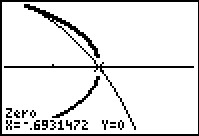
\includegraphics[width=2in]{./MatricesGraphics/NONLINEAR01.jpg} &

\hspace{0.75in} 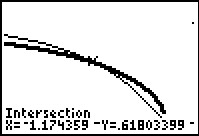
\includegraphics[width=2in]{./MatricesGraphics/NONLINEAR02.jpg}  \\

\end{tabular}

The graphs of $y = 1 - 4e^{2x}$ and \boldmath $y = \pm \sqrt{1-2e^{x}}$.

\end{center}

\item  Our last system involves three variables and gives some insight on how to keep such systems organized.  Labeling the equations as before, we have

\[\left\{\begin{array}{lrcl}   E1 & z(x-2) & = & x \\ E2 & yz & = & y \\ E3 & (x-2)^2+y^2 & = & 1 \end{array} \right.\]

The easiest equation to start with appears to be $E2$.  While it may be tempting to divide both sides of $E2$ by $y$, we caution against this practice because it presupposes $y \neq 0$.  Instead, we take $E2$ and rewrite it as $yz-y = 0$ so $y(z-1) = 0$.  From this, we get two cases:  $y = 0$ or $z = 1$.  We take each case in turn.

{ \sc Case 1: $y = 0$. }  Substituting $y=0$ into $E1$ and $E3$, we get 

\[\left\{\begin{array}{lrcl}   E1 & z(x-2) & = & x \\ E3 & (x-2)^2 & = & 1 \end{array} \right.\]

Solving $E3$ for $x$ gives $x = 1$ or $x=3$.  Substituting these values into $E1$ gives $z=-1$ when $x=1$ and $z = 3$ when $x=3$.  We obtain two solutions, $(1,0,-1)$ and $(3,0,3)$.

{ \sc Case 2:  $z = 1$. }  Substituting $z=1$ into $E1$ and $E3$ gives us 


\[\left\{\begin{array}{lrcl}   E1 & (1)(x-2) & = & x  \\ E3 & (1-2)^2+y^2 & = & 1 \end{array} \right.\]

Equation $E1$ gives us $x-2 = x$ or $-2 = 0$, which is a contradiction.  This means we have no solution to the system in this case, even though $E3$ is solvable and gives $y=0$.  Hence, our final answer is $\left\{ (1,0,-1), (3,0,3) \right\}$.  These points are easy enough to check algebraically in our three original equations, so that is left to the reader.  As for verifying these solutions graphically, they require plotting surfaces in three dimensions and looking for intersection points.  While this is beyond the scope of this book, we provide a snapshot of the graphs of our three equations near one of the solution points,  $(1,0,-1)$.

\centerline{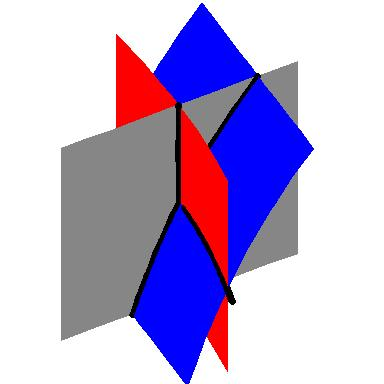
\includegraphics[height=1.75in]{./MatricesGraphics/NONLINEAR03.jpg}}

\end{enumerate}

\qed

\end{ex}

Example \ref{nonlinearex2} showcases some of the ingenuity and tenacity mentioned at the beginning of the section.  Sometimes you just have to look at a system the right way to find the most efficient method to solve it.  Sometimes you just have to try something.  

\smallskip

We close this section discussing how non-linear inequalities \index{inequality ! non-linear} can be used to describe regions in the plane which we  first introduced in Section \ref{Inequalities}.  Before we embark on some examples,  a little motivation is in order.  Suppose we wish to solve $x^2 < 4 - y^2$.  If we mimic the algorithms for solving nonlinear inequalities in one variable, we would gather all of the terms on one side and leave a $0$ on the other to obtain $x^2 + y^2 -4 < 0$.  Then we would find the zeros of the left hand side, that is, where is $x^2 + y^2 - 4 = 0$, or $x^2 + y^2 = 4$.  Instead of obtaining a few \textit{numbers} which divide the real number \textit{line} into \textit{intervals}, we get an equation of a \textit{curve}, in this case, a circle, which divides the \textit{plane} into two \textit{regions} - the `inside' and `outside' of the circle - with the circle itself as the boundary between the two.  Just like we used test \textit{values} to determine whether or not an interval belongs to the solution of the inequality, we use test \textit{points} in the each of the regions to see which of these belong to our solution set.\footnote{The theory behind why all this works is, surprisingly, the same theory which guarantees that sign diagrams work the way they do - continuity and the Intermediate Value Theorem - but in this case, applied to functions of more than one variable.}  We choose $(0,0)$ to represent the region inside the circle and $(0,3)$ to represent the points outside of the circle. When we substitute $(0,0)$ into $x^2 + y^2 -4 < 0$, we get $-4 < 4$ which is true.  This means $(0,0)$ and all the other points inside the circle are part of the solution.  On the other hand, when we substitute $(0,3)$ into the same inequality, we get $5 < 0$ which is false.  This means $(0,3)$ along with all other points outside the circle are not part of the solution.  What about points on the circle itself?  Choosing a point on the circle, say $(0,2)$, we get $0 < 0$, which means the circle itself does not satisfy the inequality.\footnote{Another way to see this is that points on the circle satisfy $x^2 + y^2 - 4 = 0$, so they do not satisfy $x^2 + y^2 - 4 < 0$.}  As a result, we leave the circle dashed in the final diagram. 

\begin{center}

\begin{mfpic}[15]{-3}{3}{-3}{3}
\fillcolor[gray]{.7}
\gfill \btwnfcn{-1.99,1.99,0.1}{0-sqrt(4-x**2)}{sqrt(4-x**2)}
\dashed \circle{(0,0),2}
\axes
\tlabel[cc](3,-0.5){\scriptsize $x$}
\tlabel[cc](0.5,3){\scriptsize $y$}
\tlabel[cc](0.5,2.25){\tiny $2$}
\tlabel[cc](0.5,-2.25){\tiny $-2$}
\xmarks{-2,-1,1,2}
\ymarks{-2,-1,1,2}
\tlpointsep{4pt}
\axislabels {x}{{\tiny $-2 \hspace{11pt}$} -2, {\tiny $\hspace{7pt} 2$} 2}
\end{mfpic}

The solution to $x^2 < 4 - y^2$

\end{center}

We put this technique to good use in the following example.

\begin{ex}  \label{nonlinearex3} Sketch the solution to the following nonlinear inequalities in the plane.

\begin{multicols}{2}

\begin{enumerate}

\item $y^2 - 4 \leq x < y+2$

\item $\left\{\begin{array}{rcr}  x^2 +y^2 & \geq & 4 \\ x^2 - 2x + y^2 - 2y & \leq & 0 \\ \end{array} \right.$

\end{enumerate}

\end{multicols}

{\bf Solution.}  

\begin{enumerate}

\item  The inequality $y^2 - 4 \leq x < y+2$ is a compound inequality.  It translates as $y^2 - 4 \leq x$ and $x < y+2$.  As usual, we solve each inequality and take the set theoretic intersection to determine the region which satisfies both inequalities.  To solve $y^2 - 4 \leq x$, we write $y^2 - x - 4 \leq 0$.  The curve $y^2 - x - 4 = 0$ describes a parabola since exactly one of the variables is squared.  Rewriting this in standard form, we get $y^2 = x+4$ and we see that the vertex is $(-4,0)$ and the parabola opens to the right.  Using the test points $(-5,0)$ and $(0,0)$, we find that the solution to the inequality includes the region to the right of, or `inside', the parabola.  The points on the parabola itself are also part of the solution, since the vertex $(-4,0)$ satisfies the inequality. We now turn our attention to $x < y+2$.  Proceeding as before, we write $x - y - 2 < 0$ and focus our attention on $x-y-2 = 0$, which is the line $y = x-2$.  Using the test points $(0,0)$ and $(0,-4)$, we find points in the region above the line $y=x-2$ satisfy the inequality. The points on the line $y = x-2$ do not satisfy the inequality, since the $y$-intercept $(0,-2)$ does not.  We see that these two regions do overlap, and to make the graph more precise, we seek the intersection of these two curves.  That is, we need to solve the system of nonlinear equations

\[\left\{\begin{array}{lrcr}  (E1) & y^2 & = & x + 4 \\ (E2) & y & = & x - 2 \\ \end{array} \right.\]

Solving $E1$ for $x$, we get $x = y^2 - 4$.  Substituting this into $E2$ gives $y = y^2 - 4 - 2$, or $y^2-y-6 = 0$.  We find $y = -2$ and $y=3$ and since $x = y^2-4$, we get that the graphs intersect at $(0,-2)$ and $(5,3)$.  Putting all of this together, we get our final answer below.

\[ \begin{array}{ccc}

\begin{mfpic}[10]{-6}{6}{-4}{4}
\fillcolor[gray]{.7}
\gfill \btwnfcn{-4,5.5,0.1}{0-sqrt(x+4)}{sqrt(x+4)}
\arrow \reverse \arrow \parafcn{-3.16,3.16,0.1}{(t^2-4,t)}
\axes
\tlabel[cc](6,-0.5){\scriptsize $x$}
\tlabel[cc](0.5,4){\scriptsize $y$}
\xmarks{-5,-4,-3,-2,-1,1,2,3,4,5}
\ymarks{-3,-2,-1,1,2,3}
\tlpointsep{4pt}
\axislabels {x}{{\tiny $-5 \hspace{7pt}$} -5,{\tiny $-4 \hspace{11pt}$} -4}
\axislabels {y}{{\tiny $-3$} -3,{\tiny $3$} 3}
\end{mfpic}

&

\hspace{.25in}

\begin{mfpic}[10]{-6}{6}{-4}{4}
\fillcolor[gray]{.7}
\gfill \btwnfcn{-2,5.5,0.1}{x-2}{3.5}
\gfill \btwnfcn{-6,-2,0.1}{-4}{3.5}
\dashed \polyline{(-2,-4), (5.5,3.5)}
\axes
\tlabel[cc](6,-0.5){\scriptsize $x$}
\tlabel[cc](0.5,4){\scriptsize $y$}
\xmarks{-5,-4,-3,-2,-1,1,2,3,4,5}
\ymarks{-3,-2,-1,1,2,3}
\tlpointsep{4pt}
\axislabels {x}{{\tiny $2$} 2, {\tiny $3$} 3,{\tiny $4$} 4,{\tiny $5$} 5}
\axislabels {y}{{\tiny $-3$} -3}
\end{mfpic} 

&

\hspace{.25in}

\begin{mfpic}[10]{-6}{6}{-4}{4}
\fillcolor[gray]{.7}
\gfill \btwnfcn{-4,0,0.1}{0-sqrt(x+4)}{sqrt(x+4)}
\gfill \btwnfcn{0,5,0.1}{x-2}{sqrt(x+4)}
\parafcn{-2,3,0.1}{(t^2-4,t)}
\dashed \polyline{(0,-2), (5,3)}
\axes
\gclear \circle{(0,-2),0.15}
\circle{(0,-2),0.15}
\gclear \circle{(5,3),0.15}
\circle{(5,3),0.15}
\tlabel[cc](6,-0.5){\scriptsize $x$}
\tlabel[cc](0.5,4){\scriptsize $y$}
\xmarks{-5,-4,-3,-2,-1,1,2,3,4,5}
\ymarks{-3,-1,1,2,3}
\tlpointsep{4pt}
\axislabels {x}{{\tiny $-5 \hspace{7pt}$} -5,{\tiny $-4 \hspace{11pt}$} -4, {\tiny $2$} 2, {\tiny $3$} 3,{\tiny $4$} 4,{\tiny $5$} 5}
\axislabels {y}{{\tiny $-3$} -3}
\end{mfpic} \\\\

y^2 - 4 \leq x & \hspace{.25in}  x < y+2 & \hspace{.25in} y^2 - 4 \leq x < y+2 \\

\end{array} \]

\item  To solve this system of inequalities, we need to find all of the points $(x,y)$ which satisfy both inequalities.  To do this, we solve each inequality separately and take the set theoretic intersection of the solution sets.  We begin with the inequality $x^2 + y^2 \geq 4$ which we rewrite as $x^2+y^2 - 4 \geq 0$.  The points which satisfy $x^2 + y^2 - 4 = 0$ form our friendly circle $x^2+y^2 = 4$.   Using test points $(0,0)$ and $(0,3)$ we find that our solution comprises the region outside the circle.  As far as the circle itself, the point $(0,2)$ satisfies the inequality, so the circle itself is part of the solution set.  Moving to the inequality $x^2 - 2x + y^2 - 2y \leq 0$, we start with $x^2 - 2x + y^2 - 2y = 0$.  Completing the squares, we obtain $(x-1)^2 + (y-1)^2 = 2$, which is a circle centered at $(1,1)$ with a radius of $\sqrt{2}$.  Choosing $(1,1)$ to represent the inside of the circle, $(1,3)$ as a point outside of the circle and $(0,0)$ as a point on the circle, we find that the solution to the inequality is the inside of the circle, including the circle itself.  Our final answer, then, consists of the points on or outside of the circle $x^2 + y^2 = 4$ which lie on or inside the circle $(x-1)^2+(y-1)^2 = 2$.  To produce the most accurate graph, we need to find where these circles intersect.  To that end, we solve the system

\[\left\{\begin{array}{lrcr}  (E1) & x^2 + y^2 & = & 4 \\ (E2) & x^2 - 2x + y^2 - 2y & = & 0 \\ \end{array} \right.\]

We can eliminate both the $x^2$ and $y^2$ by replacing $E2$ with $-E1 + E2$.  Doing so produces $-2x - 2y = -4$.  Solving this for $y$, we get $y = 2-x$.  Substituting this into $E1$ gives $x^2 + (2-x)^2 = 4$ which simplifies to $x^2 + 4-4x+x^2 = 4$ or $2x^2 - 4x = 0$.  Factoring yields $2x(x-2)$ which gives $x=0$ or $x=2$.  Substituting these values into $y=2-x$ gives the points $(0,2)$ and $(2,0)$.  The intermediate graphs and final solution are below.


\[ \begin{array}{ccc}

\begin{mfpic}[15]{-4}{4}{-4}{4}
\fillcolor[gray]{.7}
\gfill \btwnfcn{-3.5,3.5,0.1}{-3.5}{3.5}
\gclear \circle{(0,0),2}
\circle{(0,0),2}
\axes
\tlabel[cc](4,-0.5){\scriptsize $x$}
\tlabel[cc](0.5,4){\scriptsize $y$}
\xmarks{-3,-2,-1,1,2,3}
\ymarks{-3,-2,-1,1,2,3}
\tlpointsep{4pt}
\axislabels {x}{{\tiny $1$} 1 }
\axislabels {y}{{\tiny $-1$} -1,{\tiny $1$} 1}
\end{mfpic}

&

\hspace{.25in}

\begin{mfpic}[15]{-4}{4}{-4}{4}
\fillcolor[gray]{.7}
\gfill \circle{(1,1),1.414}
\axes
\circle{(1,1),1.414}
\tlabel[cc](4,-0.5){\scriptsize $x$}
\tlabel[cc](0.5,4){\scriptsize $y$}
\xmarks{-3,-2,-1,1,2,3}
\ymarks{-3,-2,-1,1,2,3}
\tlpointsep{4pt}
\axislabels {x}{{\tiny $-3 \hspace{7pt}$} -3,{\tiny $-2 \hspace{7pt}$} -2,{\tiny $-1 \hspace{7pt}$} -1, {\tiny $\hspace{7pt} 2$} 2}
\axislabels {y}{{\tiny $-3$} -3,{\tiny $-2$} -2,{\tiny $-1$} -1,{\tiny $2$} 2,{\tiny $3$} 3}
\end{mfpic}

&

\hspace{.25in}

\begin{mfpic}[15]{-4}{4}{-4}{4}
\fillcolor[gray]{.7}
\gfill \circle{(1,1),1.414}
\circle{(1,1),1.414}
\gclear \circle{(0,0),2}
\arc[s]{(2,0),(0,2),90} 
\axes
\tlabel[cc](4,-0.5){\scriptsize $x$}
\tlabel[cc](0.5,4){\scriptsize $y$}
\xmarks{-3,-2,-1,1,2,3}
\ymarks{-3,-2,-1,1,2,3}
\tlpointsep{4pt}
\axislabels {x}{{\tiny $-3 \hspace{7pt}$} -3,{\tiny $-2 \hspace{7pt}$} -2,{\tiny $-1 \hspace{7pt}$} -1, {\tiny $\hspace{7pt} 2$} 2}
\axislabels {y}{{\tiny $-3$} -3,{\tiny $-2$} -2,{\tiny $-1$} -1,{\tiny $2$} 2,{\tiny $3$} 3}
\end{mfpic} \\

x^2+y^2 \geq 4 & \hspace{.25in} x^2 - 2x + y^2 - 2y \leq 0  & \hspace{.25in} \text{Solution to the system.} \\

\end{array} \]

\qed

\end{enumerate}

\end{ex}

\newpage

\subsection{Exercises}

In Exercises \ref{solvenonlin1first} - \ref{solvenonlin1last}, solve the given system of nonlinear equations.  Sketch the graph of both equations on the same set of axes to verify the solution set. 

\begin{multicols}{3}
\begin{enumerate}

\item $\left\{\begin{array}{rcr}  x^2 - y & = & 4 \\ x^{2} + y^{2} & = & 4 \\ \end{array} \right.$ \label{solvenonlin1first}
\item $\left\{\begin{array}{rcr}  x^{2} + y^{2} & = & 4 \\ x^2 - y & = & 5 \\ \end{array} \right.$
\item $\left\{\begin{array}{rcr}  x^2+y^2 & = & 16 \\ 16x^{2} + 4y^{2} & = & 64 \\ \end{array} \right.$

\setcounter{HW}{\value{enumi}}
\end{enumerate}
\end{multicols}

\begin{multicols}{3}
\begin{enumerate}
\setcounter{enumi}{\value{HW}}

\item $\left\{\begin{array}{rcr}  x^2+y^2 & = & 16 \\ 9x^{2} - 16y^{2} & = & 144 \\ \end{array} \right.$
\item $\left\{\begin{array}{rcr}  x^2+y^2 & = & 16 \\ \frac{1}{9} y^2 - \frac{1}{16} x^2& = & 1 \\ \end{array} \right.$
\item $\left\{\begin{array}{rcr}  x^{2} + y^{2} & = & 16 \\ x-y & = & 2 \\ \end{array} \right.$ \label{solvenonlin1last}

\setcounter{HW}{\value{enumi}}
\end{enumerate}
\end{multicols}

In Exercises \ref{solvenonlin2first} - \ref{solveninlin2last}, solve the given system of nonlinear equations.  Use a graph to help you avoid any potential extraneous solutions.


\begin{multicols}{3}
\begin{enumerate}
\setcounter{enumi}{\value{HW}}


\item $\left\{\begin{array}{rcr}  x^{2} - y^{2} & = & 1 \\ x^{2} + 4y^{2} & = & 4 \\ \end{array} \right.$
\item $\left\{\begin{array}{rcr}  \sqrt{x + 1} - y & = & 0 \\ x^{2} + 4y^{2} & = & 4 \\ \end{array} \right.$
\item $\left\{\begin{array}{rcr}  x + 2y^{2} & = & 2 \\ x^{2} + 4y^{2} & = & 4 \\ \end{array} \right.$ \label{solvenonlin2first}

\setcounter{HW}{\value{enumi}}
\end{enumerate}
\end{multicols}

\begin{multicols}{3}
\begin{enumerate}
\setcounter{enumi}{\value{HW}}

\item $\left\{\begin{array}{rcr}  (x - 2)^{2} + y^{2} & = & 1 \\ x^{2} + 4y^{2} & = & 4 \\ \end{array} \right.$
\item $\left\{\begin{array}{rcr}  x^{2} + y^{2} & = & 25 \\ y - x & = & 1 \\ \end{array} \right.$
\item $\left\{\begin{array}{rcr}  x^{2} + y^{2} & = & 25 \\ x^{2} + (y - 3)^{2} & = & 10 \\ \end{array} \right.$

\setcounter{HW}{\value{enumi}}
\end{enumerate}
\end{multicols}

\begin{multicols}{3}
\begin{enumerate}
\setcounter{enumi}{\value{HW}}

\item $\left\{\begin{array}{rcr}  y & = & x^{3} + 8 \\ y & = & 10x - x^{2} \\ \end{array} \right. \vphantom{\left\{\begin{array}{rcr}  x^{2} + y^{2} & = & 25 \\ 4x^{2} - 9y & = & 0 \\ 3y^{2} - 16x & = & 0\end{array} \right.}$

\item $\left\{\begin{array}{rcr}  x^2 - xy & = & 8 \\  y^2 - xy & = & 8 \\ \end{array} \right. \vphantom{\left\{\begin{array}{rcr}  x^{2} + y^{2} & = & 25 \\ 4x^{2} - 9y & = & 0 \\ 3y^{2} - 16x & = & 0\end{array} \right.}$

\item $\left\{\begin{array}{rcr}  x^{2} + y^{2} & = & 25 \\ 4x^{2} - 9y & = & 0 \\ 3y^{2} - 16x & = & 0\end{array} \right.$ \label{solveninlin2last}

\setcounter{HW}{\value{enumi}}
\end{enumerate}
\end{multicols}

\begin{enumerate}
\setcounter{enumi}{\value{HW}}

\item  A certain bacteria culture follows the Law of Uninbited Growth, Equation \ref{lawofuninhibitedgrowth}.  After 10 minutes, there are 10,000 bacteria. Five minutes later, there are 14,000 bacteria.  How many bacteria were present initially?  How long before there are 50,000 bacteria?


\setcounter{HW}{\value{enumi}}
\end{enumerate}


Consider the system of nonlinear equations  below \[\left\{\begin{array}{rcr}  \dfrac{4}{x} + \dfrac{3}{y} & = & 1 \\[10pt] \dfrac{3}{x} + \dfrac{2}{y} & = & -1 \\ \end{array} \right.\]  If we let $u = \frac{1}{x}$ and $v = \frac{1}{y}$ then the system becomes \[\left\{\begin{array}{rcr}  4u + 3v & = & 1 \\ 3u + 2v & = & -1 \\ \end{array} \right.\] This associated system of linear equations can then be solved using any of the techniques presented earlier in the chapter to find that $u = -5$ and $v = 7$.  Thus $x = \frac{1}{u} = -\frac{1}{5}$ and $y = \frac{1}{v} = \frac{1}{7}$.  

\smallskip

We say that the original system is {\bf linear in form} \index{system of equations ! linear in form} because its equations are not linear but a few substitutions reveal a structure that we can treat like a system of linear equations.  Each system in Exercises \ref{linearformfirst} - \ref{linearformlast}  is linear in form.  Make the appropriate substitutions and solve for $x$ and $y$.

\begin{multicols}{3}
\begin{enumerate}
\setcounter{enumi}{\value{HW}}

\item $\left\{\begin{array}{rcr}  4x^{3} + 3\sqrt{y} & = & 1 \\ 3x^{3} + 2\sqrt{y} & = & -1  \end{array} \right.$ \label{linearformfirst}
\item $\left\{\begin{array}{rcr}  4e^{x} + 3e^{-y} & = & 1 \\ 3e^{x} + 2e^{-y} & = & -1  \end{array} \right.$
\item $\left\{\begin{array}{rcr}  4\ln(x) + 3y^{2} & = & 1 \\ 3\ln(x) + 2y^{2} & = & -1 \end{array} \right.$ \label{linearformlast}

\setcounter{HW}{\value{enumi}}
\end{enumerate}
\end{multicols}

\begin{enumerate}
\setcounter{enumi}{\value{HW}}

\item Solve the following system \[\left\{\begin{array}{rcr}  x^{2} + \sqrt{y} + \log_{2}(z) & = & 6 \\[3pt] 3x^{2} - 2\sqrt{y} + 2\log_{2}(z) & = & 5 \\[3pt] -5x^{2} + 3\sqrt{y} + 4\log_{2}(z) & = & 13 \end{array} \right.\]

\setcounter{HW}{\value{enumi}}
\end{enumerate}


In Exercises \ref{nonlinearsysineqfirst} - \ref{nonlinearsysineqlast}, sketch the solution to each system of nonlinear inequalities in the plane.


\begin{multicols}{2}
\begin{enumerate}
\setcounter{enumi}{\value{HW}}


\item $\left\{\begin{array}{rcr}  x^{2} - y^{2} & \leq & 1 \\ x^{2} + 4y^{2} & \geq & 4  \end{array} \right.$ \label{nonlinearsysineqfirst}
\item $\left\{\begin{array}{rcr}  x^{2} + y^{2} & < & 25 \\ x^{2} + (y - 3)^{2} & \geq & 10  \end{array} \right.$

\setcounter{HW}{\value{enumi}}
\end{enumerate}
\end{multicols}

\begin{multicols}{2}
\begin{enumerate}
\setcounter{enumi}{\value{HW}}

\item $\left\{\begin{array}{rcr}  (x - 2)^{2} + y^{2} & < & 1 \\ x^{2} + 4y^{2} & < & 4  \end{array} \right.$
\item $\left\{\begin{array}{rcr}  y & > & 10x - x^{2} \\ y & < & x^{3} + 8  \end{array} \right.$

\setcounter{HW}{\value{enumi}}
\end{enumerate}
\end{multicols}

\begin{multicols}{2}
\begin{enumerate}
\setcounter{enumi}{\value{HW}}

\item $\left\{\begin{array}{rcr}  x + 2y^{2} & > & 2 \\ x^{2} + 4y^{2} & \leq & 4  \end{array} \right.$
\item $\left\{\begin{array}{rcr}  x^{2} + y^{2} & \geq & 25 \\ y - x & \leq & 1  \end{array} \right.$ \label{nonlinearsysineqlast}

\setcounter{HW}{\value{enumi}}
\end{enumerate}
\end{multicols}

\begin{enumerate}
\setcounter{enumi}{\value{HW}}


\item Systems of nonlinear equations show up in third semester Calculus in the midst of some really cool problems.  The system below came from a problem in which we were asked to find the dimensions of a rectangular box with a volume of 1000 cubic inches that has minimal surface area.  The variables $x$, $y$ and $z$ are the dimensions of the box and $\lambda$ is called a Lagrange multiplier.  With the help of your classmates, solve the system.\footnote{If using $\lambda$ bothers you, change it to $w$ when you solve the system.} \[\left\{\begin{array}{rcr}  2y + 2z & = & \lambda yz  \\ 2x + 2z & = & \lambda xz \\ 2y + 2x & = & \lambda xy \\ xyz & = & 1000 \end{array} \right.\]

\item According to Theorem \ref{realfactorization} in Section \ref{ComplexZeros}, the polynomial $p(x) = x^{4} + 4$ can be factored into the product linear and irreducible quadratic factors.  In this exercise, we present a method for obtaining that factorization.  
\label{factorpolywithnonlinear}

\begin{enumerate}

\item Show that $p$ has no real zeros.  

\item Because $p$ has no real zeros, its factorization must be of the form $(x^{2} + ax + b)(x^{2} + cx + d)$ where each factor is an irreducible quadratic.  Expand this quantity and gather like terms together.

\item Create and solve the system of nonlinear equations which results from equating the coefficients of the expansion found above with those of $x^{4} + 4$.  You should get four equations in the four unknowns $a$, $b$, $c$ and $d$.  Write $p(x)$ in factored form.

\end{enumerate}

\item Factor $q(x) = x^{4} + 6x^{2} - 5x + 6$.

\end{enumerate}

\newpage

\subsection{Answers}

\begin{multicols}{2}
\begin{enumerate}

\item $(\pm 2, 0)$, $\left(\pm \sqrt{3}, -1\right)$ \\
\begin{mfpic}[15]{-3}{3}{-5}{3}
\arrow \reverse \arrow \function{-2.5,2.5,0.1}{x**2 - 4}
\circle{(0,0),2}
\point[3pt]{(2,0), (-2,0), (1.7320,-1), (-1.7320,-1)}
\axes
\tlabel[cc](3,-0.5){\scriptsize $x$}
\tlabel[cc](0.5,3){\scriptsize $y$}
\xmarks{-2,-1,1,2}
\ymarks{-4,-3,-2,-1,1,2}
\tlpointsep{4pt}
\tiny
\axislabels {x}{{$-2 \hspace{7pt}$} -2, {$-1 \hspace{7pt}$} -1, {$1$} 1, {$2$} 2}
\axislabels {y}{{$-4$} -4,{$-3$} -3,{$-2$} -2, {$-1$} -1, {$1$} 1, {$2$} 2}
\normalsize
\end{mfpic}

\vfill

\columnbreak

\item No solution \\

\begin{mfpic}[15]{-3}{3}{-6}{3}
\arrow \reverse \arrow \function{-2.75,2.75,0.1}{x**2 - 5}
\circle{(0,0),2}
\axes
\tlabel[cc](3,-0.5){\scriptsize $x$}
\tlabel[cc](0.5,3){\scriptsize $y$}
\xmarks{-2,-1,1,2}
\ymarks{-4,-3,-2,-1,1,2}
\tlpointsep{4pt}
\tiny
\axislabels {x}{{$-2 \hspace{7pt}$} -2, {$-1 \hspace{7pt}$} -1, {$1$} 1, {$2$} 2}
\axislabels {y}{{$-4$} -4,{$-3$} -3,{$-2$} -2, {$-1$} -1, {$1$} 1, {$2$} 2}
\normalsize
\end{mfpic}

\setcounter{HW}{\value{enumi}}
\end{enumerate}
\end{multicols}

\begin{multicols}{2}
\begin{enumerate}
\setcounter{enumi}{\value{HW}}

\item  $(0, \pm 4)$ \\
\begin{mfpic}[10]{-5}{5}{-5}{5}
\ellipse{(0,0), 2, 4}
\circle{(0,0),4}
\point[3pt]{(0,4), (0,-4)}
\axes
\tlabel[cc](5,-0.5){\scriptsize $x$}
\tlabel[cc](0.5,5){\scriptsize $y$}
\xmarks{-4,-3,-2,-1,1,2,3,4}
\ymarks{-4,-3,-2,-1,1,2,3,4}
\tlpointsep{4pt}
\tiny
\axislabels {x}{{$-4 \hspace{7pt}$} -4,{$-3 \hspace{7pt}$} -3,{$-2 \hspace{7pt}$} -2, {$-1 \hspace{7pt}$} -1, {$1$} 1, {$2$} 2, {$3$} 3, {$4$} 4}
\axislabels {y}{{$-4$} -4,{$-3$} -3,{$-2$} -2, {$-1$} -1, {$1$} 1, {$2$} 2, {$3$} 3, {$4$} 4}
\normalsize
\end{mfpic}

\vfill

\columnbreak

\item  $(\pm 4,0)$ \\
\begin{mfpic}[10]{-7}{7}{-5}{5}
\arrow \reverse \arrow \parafcn{-1, 1,0.1}{(4*cosh(t), 3*sinh(t))}
\arrow \reverse \arrow \parafcn{-1, 1,0.1}{(0-4*cosh(t), 3*sinh(t))}
\circle{(0,0),4}
\point[3pt]{(4,0), (-4,0)}
\axes
\tlabel[cc](7,-0.5){\scriptsize $x$}
\tlabel[cc](0.5,5){\scriptsize $y$}
\xmarks{-6,-5,-4,-3,-2,-1,1,2,3,4,5,6}
\ymarks{-4,-3,-2,-1,1,2,3,4}
\tlpointsep{4pt}
\tiny
\axislabels {x}{{$-6 \hspace{7pt}$} -6,{$-5 \hspace{7pt}$} -5,{$-4 \hspace{7pt}$} -4,{$-3 \hspace{7pt}$} -3,{$-2 \hspace{7pt}$} -2, {$-1 \hspace{7pt}$} -1, {$1$} 1, {$2$} 2, {$3$} 3, {$4$} 4, {$5$} 5, {$6$} 6}
\axislabels {y}{{$-4$} -4,{$-3$} -3,{$-2$} -2, {$-1$} -1, {$1$} 1, {$2$} 2, {$3$} 3, {$4$} 4}
\normalsize
\end{mfpic}


\setcounter{HW}{\value{enumi}}
\end{enumerate}
\end{multicols}

\begin{multicols}{2}
\begin{enumerate}
\setcounter{enumi}{\value{HW}}

\item  $\left(\pm \frac{4 \sqrt{7}}{5}, \pm \frac{12 \sqrt{2}}{5}  \right)$ \\
\begin{mfpic}[10]{-5}{5}{-5}{5}
\arrow \reverse \arrow \parafcn{-1, 1,0.1}{(4*sinh(t), 3*cosh(t))}
\arrow \reverse \arrow \parafcn{-1, 1,0.1}{(4*sinh(t), 0-3*cosh(t))}
\circle{(0,0),4}
\point[3pt]{(2.1166,3.3941), (2.1166, -3.3941), (-2.1166,3.3941), (-2.1166,-3.3941) }
\axes
\tlabel[cc](5,-0.5){\scriptsize $x$}
\tlabel[cc](0.5,5){\scriptsize $y$}
\xmarks{-4,-3,-2,-1,1,2,3,4}
\ymarks{-4,-3,-2,-1,1,2,3,4}
\tlpointsep{4pt}
\tiny
\axislabels {x}{{$-4 \hspace{7pt}$} -4,{$-3 \hspace{7pt}$} -3,{$-2 \hspace{7pt}$} -2, {$-1 \hspace{7pt}$} -1, {$1$} 1, {$2$} 2, {$3$} 3, {$4$} 4}
\axislabels {y}{{$-4$} -4,{$-3$} -3,{$-2$} -2, {$-1$} -1, {$1$} 1, {$2$} 2, {$3$} 3, {$4$} 4}
\normalsize
\end{mfpic}

\vfill

\columnbreak

\item  $\left( 1 + \sqrt{7}, -1 + \sqrt{7}  \right)$, $\left( 1 - \sqrt{7}, -1 - \sqrt{7}  \right)$ \\
\begin{mfpic}[10]{-5}{5}{-5}{5}
\arrow \reverse \arrow \function{-3,5,0.1}{x-2}
\circle{(0,0),4}
\point[3pt]{(3.6458,1.6458), (-1.6458, -3.6458) }
\axes
\tlabel[cc](5,-0.5){\scriptsize $x$}
\tlabel[cc](0.5,5){\scriptsize $y$}
\xmarks{-4,-3,-2,-1,1,2,3,4}
\ymarks{-4,-3,-2,-1,1,2,3,4}
\tlpointsep{4pt}
\tiny
\axislabels {x}{{$-4 \hspace{7pt}$} -4,{$-3 \hspace{7pt}$} -3,{$-2 \hspace{7pt}$} -2, {$-1 \hspace{7pt}$} -1, {$1$} 1, {$2$} 2, {$3$} 3, {$4$} 4}
\axislabels {y}{{$-4$} -4,{$-3$} -3,{$-2$} -2, {$-1$} -1, {$1$} 1, {$2$} 2, {$3$} 3, {$4$} 4}
\normalsize
\end{mfpic}

\setcounter{HW}{\value{enumi}}
\end{enumerate}
\end{multicols}

\begin{multicols}{3}
\begin{enumerate}
\setcounter{enumi}{\value{HW}}

\item $\left( \pm \frac{2 \sqrt{10}}{5}, \pm \frac{\sqrt{15}}{5} \right)$
\item $(0, 1)$
\item $(0, \pm 1), \; (2, 0)$


\setcounter{HW}{\value{enumi}}
\end{enumerate}
\end{multicols}

\begin{multicols}{3}
\begin{enumerate}
\setcounter{enumi}{\value{HW}}
\item $\left( \frac{4}{3}, \pm \frac{\sqrt{5}}{3} \right)$
\item $(3, 4), \; (-4, -3)$
\item $(\pm 3, 4)$
\setcounter{HW}{\value{enumi}}
\end{enumerate}
\end{multicols}

\begin{multicols}{3}
\begin{enumerate}
\setcounter{enumi}{\value{HW}}

\item $(-4, -56), \; (1, 9), \; (2, 16)$
\item $(-2,2)$, $(2,-2)$
\item $(3, 4)$

\setcounter{HW}{\value{enumi}}
\end{enumerate}
\end{multicols}


\begin{enumerate}
\setcounter{enumi}{\value{HW}}

\item  Initially, there are $\frac{250000}{49} \approx 5102$ bacteria.  It will take $\frac{5\ln(49/5)}{\ln(7/5)} \approx 33.92$ minutes for the colony to grow to 50,000 bacteria.

\setcounter{HW}{\value{enumi}}
\end{enumerate}


\begin{multicols}{3}
\begin{enumerate}
\setcounter{enumi}{\value{HW}}

\item $\left( -\sqrt[3]{5}, 49 \right)$
\item No solution
\item $\left( e^{-5}, \pm \sqrt{7} \right)$

\setcounter{HW}{\value{enumi}}
\end{enumerate}
\end{multicols}

\begin{enumerate}
\setcounter{enumi}{\value{HW}}

\item $(1, 4, 8), \; (-1, 4, 8)$


\setcounter{HW}{\value{enumi}}
\end{enumerate}


\begin{multicols}{2}
\begin{enumerate}
\setcounter{enumi}{\value{HW}}

\item $\left\{\begin{array}{rcr}  x^{2} - y^{2} & \leq & 1 \\ x^{2} + 4y^{2} & \geq & 4  \end{array} \right.$ \\

\begin{mfpic}[15]{-3}{3}{-3}{3}
\fillcolor[gray]{.7}
\gfill \rect{(-2.8,-2.8),(2.8,2.8)}
\gclear \btwnfcn{-3,-1,0.1}{sqrt((x**2) - 1)}{-sqrt((x**2) - 1)}
\gclear \btwnfcn{1,3,0.1}{sqrt((x**2) - 1)}{-sqrt((x**2) - 1)}
\gclear \btwnfcn{-2,2,0.1}{sqrt(1 - ((x**2)/4))}{-sqrt(1 - ((x**2)/4))}
\function{-1.2649,1.2649,0.1}{sqrt(1 - ((x**2)/4))}
\function{-1.2649,1.2649,0.1}{-sqrt(1 - ((x**2)/4))}
\arrow \reverse \function{-3,-1.2649,0.1}{sqrt((x**2) - 1)}
\arrow \reverse \function{-3,-1.2649,0.1}{-sqrt((x**2) - 1)}
\arrow \function{1.2649,3,0.1}{sqrt((x**2) - 1)}
\arrow \function{1.2649,3,0.1}{-sqrt((x**2) - 1)}
\axes
\tlabel[cc](3,-0.5){\scriptsize $x$}
\tlabel[cc](0.5,3){\scriptsize $y$}
\xmarks{-2,-1,1,2}
\ymarks{-2,-1,1,2}
\tlpointsep{4pt}
\tiny
\axislabels {x}{{$-2 \hspace{7pt}$} -2, {$-1 \hspace{7pt}$} -1, {$1$} 1, {$2$} 2}
\axislabels {y}{{$-2$} -2, {$-1$} -1, {$1$} 1, {$2$} 2}
\normalsize
\end{mfpic}

\vfill

\columnbreak

\item $\left\{\begin{array}{rcr}  x^{2} + y^{2} & < & 25 \\ x^{2} + (y - 3)^{2} & \geq & 10  \end{array} \right.$\\

\begin{mfpic}[10]{-6}{6}{-6}{5}
\fillcolor[gray]{.7}
\gfill \circle{(0,0),5}
\dashed \circle{(0,0),5}
\gclear \circle{(0,3),3.16228}
\arc[t]{(-3,4),(0,-0.166228),(3,4)}
\gclear \circle{(3,4),0.15}
\circle{(3,4),0.15}
\gclear \circle{(-3,4),0.15}
\circle{(-3,4),0.15}
\axes
\tlabel[cc](6,-0.5){\scriptsize $x$}
\tlabel[cc](0.5,5){\scriptsize $y$}
\xmarks{-5 step 1 until 5}
\ymarks{-5 step 1 until 4}
\tlpointsep{4pt}
\tiny
\axislabels {x}{{$-5 \hspace{7pt}$} -5, {$-4 \hspace{7pt}$} -4, {$-3 \hspace{7pt}$} -3, {$-2 \hspace{7pt}$} -2, {$-1 \hspace{7pt}$} -1, {$1$} 1, {$2$} 2, {$3$} 3, {$4$} 4, {$5$} 5}
\axislabels {y}{{$-5$} -5, {$-4$} -4, {$-3$} -3, {$-2$} -2, {$-1$} -1, {$1$} 1, {$2$} 2, {$3$} 3, {$4$} 4}
\normalsize
\end{mfpic}

\setcounter{HW}{\value{enumi}}
\end{enumerate}
\end{multicols}

\begin{multicols}{2}
\begin{enumerate}
\setcounter{enumi}{\value{HW}}

\item $\left\{\begin{array}{rcr}  (x - 2)^{2} + y^{2} & < & 1 \\ x^{2} + 4y^{2} & < & 4  \end{array} \right.$ \\

\begin{mfpic}[30]{0}{2.75}{-1.5}{1.5}
\fillcolor[gray]{.7}
\gfill \circle{(2,0),1}
\gclear \btwnfcn{1.3333,2,0.1}{sqrt(1 - ((x**2)/4))}{sqrt(1 - ((x - 2)**2))}
\gclear \btwnfcn{1.3333,2,0.1}{-sqrt(1 - ((x**2)/4))}{-sqrt(1 - ((x - 2)**2))}
\gclear \btwnfcn{2,3,0.1}{-sqrt(1 - ((x - 2)**2))}{sqrt(1 - ((x - 2)**2))}
\gclear \rect{(2.5,-1),(3,1)}
\drawcolor{white} \arc[t]{(1.3333,-0.745356),(3,0),(1.3333,0.745356)}
\drawcolor{white} \polyline{(2,-1),(2,1)}
\drawcolor{black}
\dashed \arc[t]{(1.3333,-0.745356),(1,0),(1.3333,0.745356)}
\dashed \parafcn{-0.84107,0.84107,0.1}{(2*cos(t),sin(t))}

\axes
\tlabel[cc](2.75,-0.25){\scriptsize $x$}
\tlabel[cc](0.25,1.5){\scriptsize $y$}
\ymarks{-1,1}
\tlpointsep{4pt}
\tiny
\axislabels {x}{{$1$} 0.9, {$2$} 2.1}
\axislabels {y}{{$-1$} -1, {$1$} 1}
\normalsize
\end{mfpic}

\vfill

\columnbreak

\item  $\left\{\begin{array}{rcr}  y & > & 10x - x^{2} \\ y & < & x^{3} + 8  \end{array} \right.$ \\

\begin{mfpic}[10][1]{-5}{7}{-28}{120}
\fillcolor[gray]{.7}
\gfill \btwnfcn{-4,1,0.1}{0.5*(10*x - (x**2))}{0.5*((x**3) + 8)}
\gfill \btwnfcn{2,6.2,0.1}{0.5*(10*x - (x**2))}{0.5*((x**3) + 8)}
\dashed \function{-4,1,0.1}{0.5*(10*x - (x**2))}
\dashed \function{-4,1,0.1}{0.5*((x**3) + 8)}
\arrow \dashed \function{2,6.2,0.1}{0.5*(10*x - (x**2))}
\arrow \dashed \function{2,6.2,0.1}{0.5*((x**3) + 8)}
\axes
\tlabel[cc](7,-4){\scriptsize $x$}
\tlabel[cc](0.5,120){\scriptsize $y$}
\xmarks{-4 step 1 until 2}
\ymarks{-28,4.5,8}
\tlpointsep{4pt}
\tiny
\axislabels {x}{{$-4 \hspace{7pt}$} -4, {$-3 \hspace{7pt}$} -3, {$-2 \hspace{7pt}$} -2, {$-1 \hspace{7pt}$} -1, {$1$} 1, {$2$} 2}
\axislabels {y}{{$-56$} -28, {$9$} 4.5, {$16$} 8}
\normalsize
\end{mfpic}

\setcounter{HW}{\value{enumi}}
\end{enumerate}
\end{multicols}

\begin{multicols}{2}
\begin{enumerate}
\setcounter{enumi}{\value{HW}}

\item $\left\{\begin{array}{rcr}  x + 2y^{2} & > & 2 \\ x^{2} + 4y^{2} & \leq & 4  \end{array} \right.$ \\

\begin{mfpic}[30]{-0.5}{2.5}{-1.5}{1.5}
\fillcolor[gray]{.7}
\gfill \btwnfcn{0,2,0.1}{sqrt(1 - (x/2))}{sqrt(1 - ((x**2)/4))}
\gfill \btwnfcn{0,2,0.1}{-sqrt(1 - (x/2))}{-sqrt(1 - ((x**2)/4))}
\parafcn{-1.5708, 1.5708,0.1}{(2*cos(t),sin(t))}
\dashed \parafcn{-1,1,0.1}{(2 - (2*(t**2)), t)}
\axes
\gclear \circle{(2,0), 0.05}
\circle{(2,0), 0.05}
\gclear \circle{(0,1), 0.05}
\circle{(0,1), 0.05}
\gclear \circle{(0,-1), 0.05}
\circle{(0,-1), 0.05}
\tlabel[cc](2.5,-0.25){\scriptsize $x$}
\tlabel[cc](0.25,1.5){\scriptsize $y$}
\xmarks{1}
\tlpointsep{4pt}
\tiny
\axislabels {x}{{$1$} 1, {$2$} 2.1}
\axislabels {y}{{$-1$} -1, {$1$} 1}
\normalsize
\end{mfpic}

\vfill

\columnbreak

\item  $\left\{\begin{array}{rcr}  x^{2} + y^{2} & \geq & 25 \\ y - x & \leq & 1  \end{array} \right.$ \\

\begin{mfpic}[6]{-7}{7}{-7}{8}
\fillcolor[gray]{.7}
\gfill \btwnfcn{-7,7,0.1}{-7}{1+x}
\gclear \circle{(0,0), 5}
\arc[t]{(-4,-3), (5,0), (3,4)}
\arrow \reverse \function{-7,-4,0.1}{1+x}
\arrow \function{3,7,0.1}{1+x}
\axes
\tlabel[cc](7,-0.5){\scriptsize $x$}
\tlabel[cc](0.5,8){\scriptsize $y$}
\xmarks{-6 step 1 until 6}
\ymarks{-6 step 1 until 7}
\tlpointsep{4pt}
\tiny
\axislabels {x}{{$-5 \hspace{7pt}$} -5,  {$-3 \hspace{7pt}$} -3,  {$-1 \hspace{7pt}$} -1, {$1$} 1,  {$3$} 3,  {$5$} 5}
\axislabels {y}{ {$-5$} -5,  {$-3$} -3,   {$1$} 1,  {$3$} 3,  {$5$} 5, {$7$} 7}
\normalsize
\end{mfpic}

\setcounter{HW}{\value{enumi}}
\end{enumerate}
\end{multicols}


\begin{enumerate}
\setcounter{enumi}{\value{HW}}

\item $x = 10, \; y = 10, \; z = 10, \lambda = \frac{2}{5}$

\setcounter{HW}{\value{enumi}}
\end{enumerate}

\begin{enumerate}
\setcounter{enumi}{\value{HW}}

\item \begin{enumerate} 

\addtocounter{enumii}{2}

\item $x^{4} + 4 = (x^{2} - 2x + 2)(x^{2} + 2x + 2)$

\end{enumerate}

\item $x^{4} + 6x^{2} - 5x + 6 = (x^{2} - x + 1)(x^{2} + x + 6)$

\end{enumerate}

\closegraphsfile